\documentclass[]{report}
\usepackage[utf8]{inputenc}
\usepackage{graphicx}

% Title Page
\title{Ghosts}
\author{Clara Bringer et Pierre Gervais}

\begin{document}
\maketitle

\section{Liste des fonctionnalités}
\subsection{Déroulement d'une partie}
\paragraph{Préparation de la partie}
\subparagraph*{}
Avant que la partie ne commence, vous êtes invités a sélectionner (ou non) le mode triche puis à choisir des extensions parmi une liste.
\subparagraph*{}
Vous pouvez faire jouer automatiquement un ou deux joueurs à l'aide d'un fichier en \textit{.gf} décrivant la disposition initiale des fantômes ainsi que les déplacements que le joueur effectuera.\\
\emph{Attention : Si un joueur automatique ne peut pas placer ses pions comme décrit dans son fichier car sa disposition est incompatible avec les règles et/ou le plateau, ou s'il ne peut pas effectuer un déplacement car celui-ci est illégal voire impossible, une exception est lancée.}

\paragraph{Placement des fantômes}
\subparagraph*{}
En cliquant sur une case, la fenêtre propose d'y placer un fantôme en choisissant :
\begin{itemize}
	\item son type, vous avez le choix parmi le type de fantôme "basique" et les éventuels autres types contenus dans les extensions sélectionnées ;
	\item s'il est bon ou mauvais.
\end{itemize}
\subparagraph*{}
Vous pouvez supprimer un pion en cliquant dessus puis en confirmant la suppression.

\paragraph{Déroulement du jeu}
\subparagraph{Déplacements}
Chaque joueur doit, pour déplacer ses pions, cliquer sur l'un de ses fantômes, puis cliquer sur la case en surbrillance où il souhaite le déposer.
\subparagraph{Fin de jeu}
Si le livre de règles indique que la partie est terminée, le jeu annonce l'éventuel gagnant (ou match nul si c'est le cas) puis ferme le programme.

\subsection{Extensions}
\subparagraph{Extension de base : \textit{BaseExtension} dans \textit{base}}
Ce package contient l'extension dite "de base", c'est à dire les règles et les pions du jeu original.

\subparagraph{Extension cavaliers : \textit{KnightsExtension} dans \textit{base.knights}}
Les cavaliers possèdent les mêmes déplacements qu'aux échecs ; deux cases dans une direction et une case dans l'autre. Ils peuvent être au nombre de $\frac{t}{2}-1$ maximum, bons et mauvais confondus, où $t$ est la taille d'un côté du plateau.

\subparagraph{Extension dames : \textit{CheckersExtension} dans \textit{base.checkers}}
Les dames possèdent les mêmes déplacements que les pions du jeu de Dames ; une case en diagonale. Chaque joueur peut en avoir au plus $t - 2$.

\subparagraph{Extension hardcore : \textit{HardcoreExtension} dans \textit{base}}
Avec cette extension, vous devez faire sortir \emph{deux} bons fantômes ou capturer tous les fantômes adverses.

\subparagraph{Extension plateau 12 par 12 cases : \textit{Boards12Per12Extension} dans \textit{base}}
Vous jouez avec un plateau de 12 par 12 cases avec une sortie dans chaque coin du camp opposé.

\subparagraph{Extension plateau spécial : \textit{SpecialBoardExtension} dans \textit{base}}
Cette extension propose un plateau de 10 par 10 cases dont les sorties sont initialement cachées par les pions adverses.\\
\emph{Cette extension n'est pas compatible avec l'extension précédente.}

\section{Diagrammes de classe}

\begin{figure}[!h]
	\caption{Diagramme de classes du package \textit{core}}
	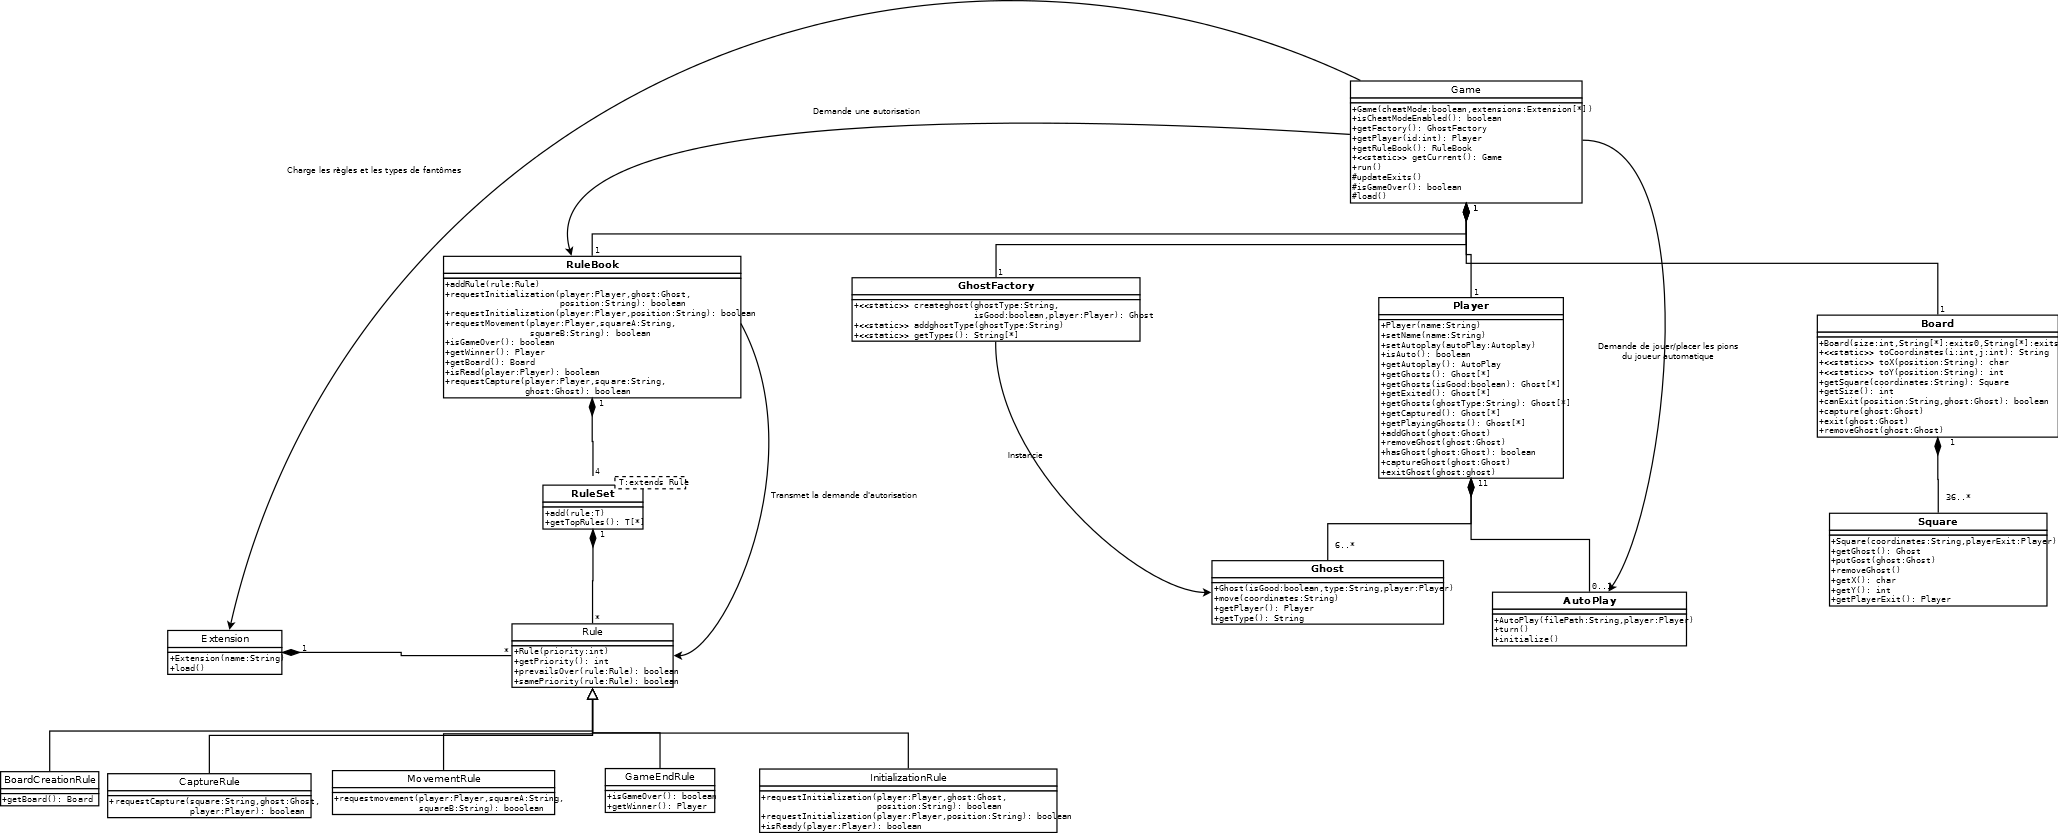
\includegraphics[width=\textwidth]{core.png}
\end{figure}

\begin{figure}[!h]
	\caption{Diagramme de classes du package \textit{core.GUIGame}}
	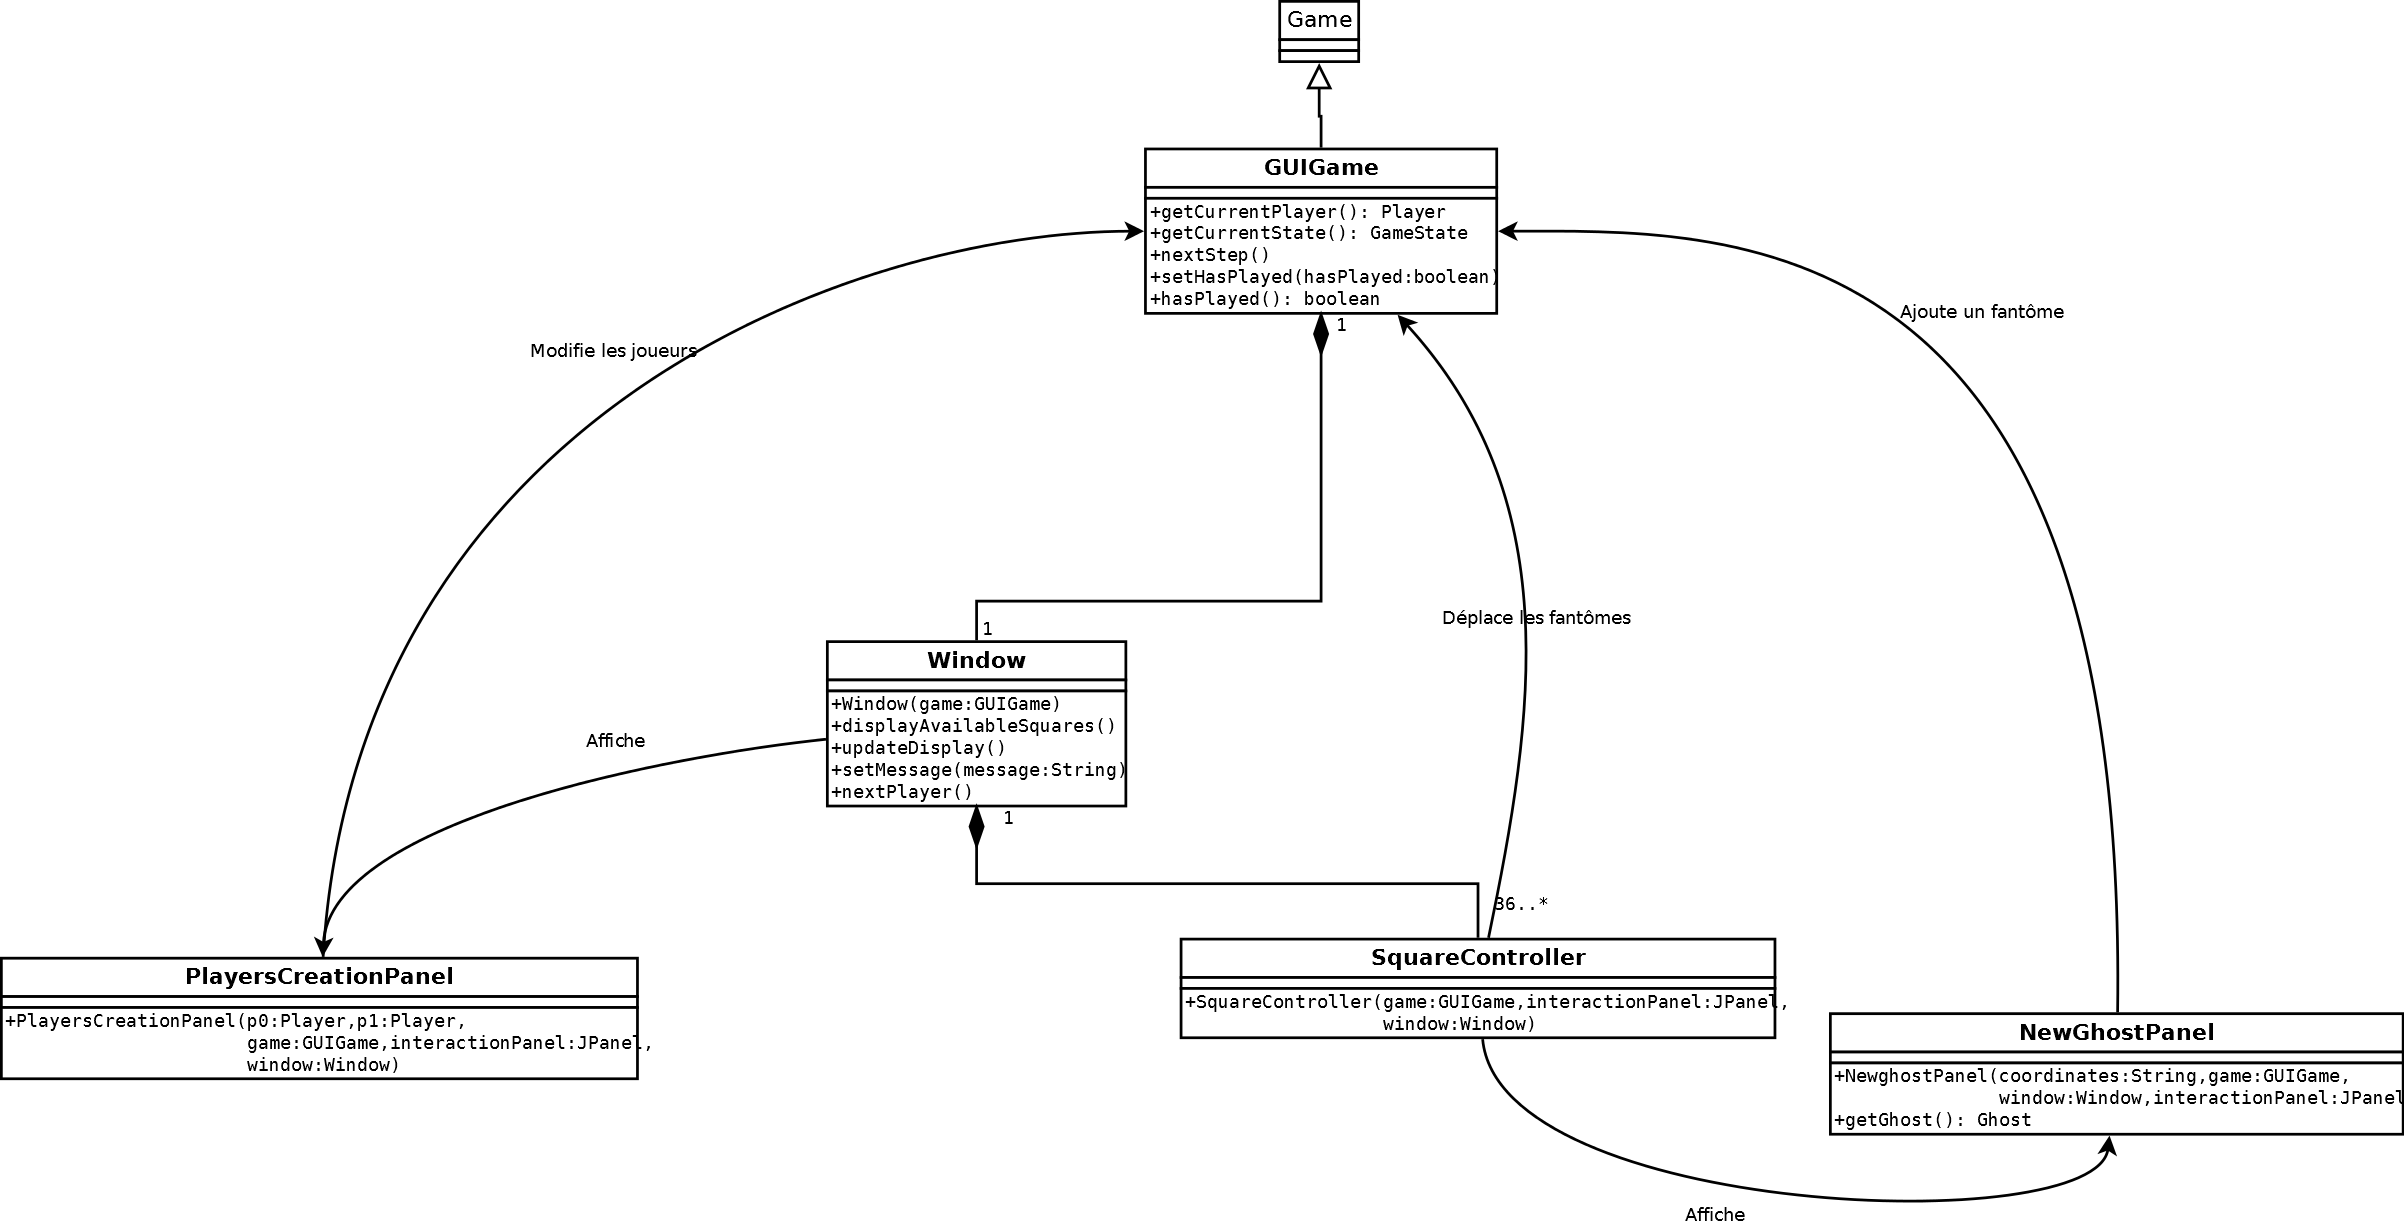
\includegraphics[width=\textwidth]{core_GUIGame.png}
\end{figure}

Les diagrammes sont disponibles depuis la doc en grand format dans la description des packages \textit{core} et \textit{core.GUIGame}.

\end{document}